\begin{problem}{데이터 제작}{표준 입력(stdin)}{표준 출력(stdout)}{1\,초}{1024\,MB}

\begin{flushright}
``정휘야, 데이터 만들어야지"
\end{flushright}

정휘는 원래 UCPC 2020 Call for Tasks에 점과 선분이 등장하는 재미있는 기하 문제를 제출하려고 했지만, 데이터를 너무 만들기 귀찮은 나머지 출제를 포기했다.
UCPC 2020에 문제를 꼭 출제하고 싶어 고민하고 있던 정휘는 아주 좋은 아이디어를 냈다. 바로 대회 참가자들에게 데이터를 만들게 하는 것이다! 원래는 정휘가 해야 할 일이었지만, 이제는 여러분이 좌표 평면상에 점 $N$개와 선분 $M$개를 적절히 배치해서 $K$개의 영역이 있는 데이터를 만들어야 한다.

영역은 평면 상의 빈 공간이며, 선분으로 모든 면이 둘러 쌓여 있어야 한다. 영역은 다른 영역으로 둘러 쌓여질 수도 있다. 좌표 범위가 너무 넓으면 계산하기 너무 힘들기 때문에, 79brue의 팬인 정휘는 모든 점의 좌표 범위를 $79$ 이하의 자연수로 제한하기로 했다!

여러분은 아래 조건을 모두 만족시키는 데이터를 만들어야 한다.

\begin{itemize}
\item 각 점의 $x$, $y$좌표는 $1$ 이상 $79$ 이하의 자연수가 되어야 한다.
\item 모든 점의 위치는 서로 달라야 한다.
\item 같은 두 점을 잇는 선분이 여러 개 존재하면 안 된다.
\item 선분은 서로 다른 두 점을 이어야 한다.
\item 서로 다른 두 선분은 끝점을 제외한 곳에서 교차하면 안 된다.
\item 선분의 양 끝점을 제외한 점은 선분 위에 있으면 안 된다.
\end{itemize}

아래에서 (a)는 점 $3$개, 선분 $3$개로 $1$개의 영역을 만든 그림이고, (b)는 점 $4$개, 선분 $6$개로 $3$개의 영역을 만든 그림이다. (c)는 곡선이 존재하기 때문에, (d)는 교차하는 선분들이 존재하기 때문에 올바르지 않은 출력이다.

\begin{figure}[h!]
\centering

\begin{subfigure}[b]{.22\textwidth}
\centering
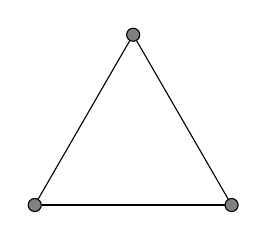
\begin{tikzpicture}[every node/.style={draw, fill=gray, scale=0.5}]
\def \h {1.25}
\node[circle] (1) at (0, 1.73*\h) {};
\node[circle] (2) at (-1*\h, 0) {};
\node[circle] (3) at (1*\h, 0) {};
\draw (1) -- (2);
\draw (2) -- (3);
\draw (1) -- (3);
\end{tikzpicture}
\caption{점 3개와 선분 3개로 영역 1개를 만든 그림}
\end{subfigure}%
\hfill
\begin{subfigure}[b]{.22\textwidth}
\centering
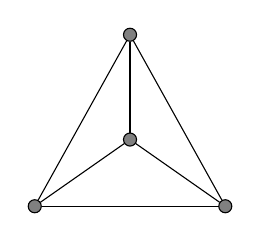
\begin{tikzpicture}[every node/.style={draw, fill=gray, scale=0.5}]
\def \h {1.21}
\node[circle] (1) at (0, 1.8*\h) {};
\node[circle] (2) at (-1*\h, 0) {};
\node[circle] (3) at (1*\h, 0) {};
\node[circle] (4) at (0, 0.7*\h) {};
\draw (1) -- (2);
\draw (2) -- (3);
\draw (1) -- (3);
\draw (1) -- (4);
\draw (2) -- (4);
\draw (3) -- (4);
\end{tikzpicture}
\caption{점 4개와 선분 6개로 영역 3개를 만든 그림}
\end{subfigure}%
\hfill
\begin{subfigure}[b]{.22\textwidth}
\centering
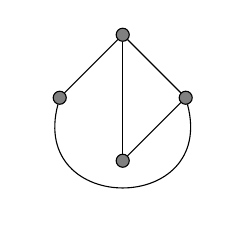
\begin{tikzpicture}[every node/.style={draw, fill=gray, scale=0.5}, font=\tiny]
\node[circle] (1) at (0, -0.8) {};
\node[circle] (2) at (0.8, 0) {};
\node[circle] (3) at (0, 0.8) {};
\node[circle] (4) at (-0.8, 0) {};
\draw (1) -- (2);
\draw (1) -- (3);
\draw (2) -- (3);
\draw (3) -- (4);
\draw (2) .. controls +(0.4, -1.5) and +(-0.4, -1.5) .. (4);
\end{tikzpicture}
\caption{곡선이 존재하여 조건에 맞지 않는 그림}
\end{subfigure}%
\hfill
\begin{subfigure}[b]{.22\textwidth}
\centering
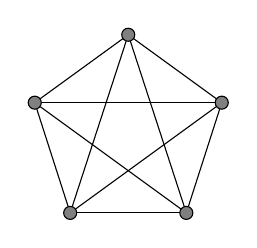
\begin{tikzpicture}[every node/.style={draw, fill=gray, scale=0.5}, font=\tiny]
\def \h {1.25}
\node[circle] (1) at (0, 1*\h) {};
\node[circle] (2) at (-0.95*\h, 0.31*\h) {};
\node[circle] (3) at (0.95*\h, 0.31*\h) {};
\node[circle] (4) at (-0.59*\h, -0.81*\h) {};
\node[circle] (5) at (0.59*\h, -0.81*\h) {};
\draw (1) -- (2);
\draw (1) -- (3);
\draw (1) -- (4);
\draw (1) -- (5);
\draw (2) -- (3);
\draw (2) -- (4);
\draw (2) -- (5);
\draw (3) -- (4);
\draw (3) -- (5);
\draw (4) -- (5);
\end{tikzpicture}
\caption{교차하는 선분이 존재해 조건에 맞지 않는 그림}
\end{subfigure}%
\end{figure}

\InputFile
첫 번째 줄에 배치해야 할 점의 개수, 선분의 개수와 만들어야 하는 영역의 개수를 나타내는 세 자연수 $N,M,K$가 주어진다. ($3 \leq N \leq 3\ 000$, $0 \leq M$, $0 \leq K$)

$N$개의 점과 $M$개의 서로 교차하지 않는 선분으로 $K$개의 다각형을 만들 수 있는 경우만 입력으로 주어진다.

\OutputFile
첫째 줄부터 $N$번째 줄까지 $i$번째 줄에 $i$번째 점의 좌표를 출력한다. $N+1$번째 줄부터 $N+M$번째 줄까지 각 선분이 몇 번째 점을 연결하는지 출력한다.

\Example

\begin{example}
\exmp{
4 6 3
}{%
1 1
3 1
2 2
2 3
1 2
1 3
1 4
2 3
2 4
3 4
}%
\exmp{
6 5 1
}{%
1 1
1 2
2 1
3 1
3 2
4 1
1 2
1 3
2 3
4 5
5 6
}%
\end{example}

\Note
\begin{figure}[h!]
\centering
\begin{subfigure}[b]{.45\textwidth}
\centering
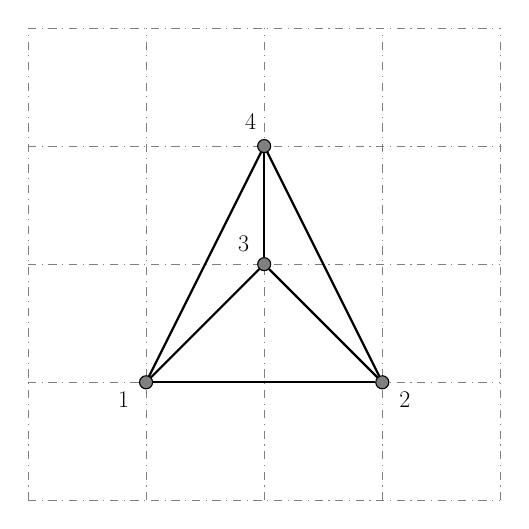
\begin{tikzpicture}[
    every node/.style={draw, scale=0.5, fill=gray, circle},
    every label/.style={draw=none, fill=none, label distance=0.15cm, font=\fontsize{16}{16}\selectfont},
]
\def \h {1.5}
\draw[step=\h,black,thin, dashdotted, help lines] (0,0) grid (4*\h,4*\h);
\node[label={-150:1}] (1) at (1*\h, 1*\h) {};
\node[label={-30:2}] (2) at (3*\h, 1*\h) {};
\node[label={135:3}] (3) at (2*\h, 2*\h) {};
\node[label={100:4}] (4) at (2*\h, 3*\h) {};
\draw[thick] (1) -- (2);
\draw[thick] (2) -- (3);
\draw[thick] (1) -- (3);
\draw[thick] (1) -- (4);
\draw[thick] (2) -- (4);
\draw[thick] (3) -- (4);


\end{tikzpicture}
\caption{예제 1에 해당하는 그림}
\end{subfigure}%
\hfill
\begin{subfigure}[b]{.45\textwidth}
\centering
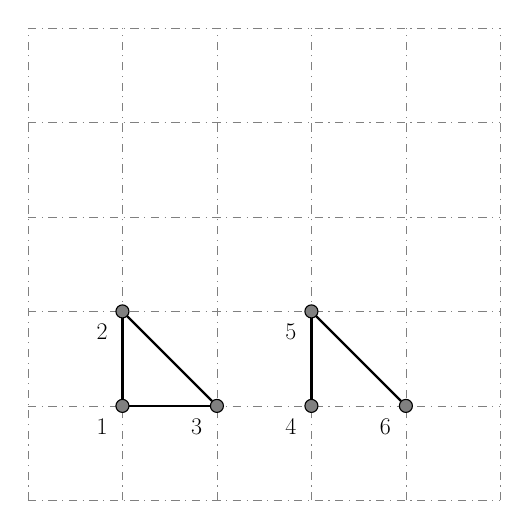
\begin{tikzpicture}[
    every node/.style={draw, scale=0.5, fill=gray, circle},
    every label/.style={draw=none, fill=none, label distance=0.15cm, font=\fontsize{16}{16}\selectfont},
]
\def \h {1.2}
\draw[step=\h,black,thin, dashdotted, help lines] (0,0) grid (5*\h,5*\h);
\node[label={-135:1}] (1) at (1*\h, 1*\h) {};
\node[label={-135:2}] (2) at (1*\h, 2*\h) {};
\node[label={-135:3}] (3) at (2*\h, 1*\h) {};
\node[label={-135:4}] (4) at (3*\h, 1*\h) {};
\node[label={-135:5}] (5) at (3*\h, 2*\h) {};
\node[label={-135:6}] (6) at (4*\h, 1*\h) {};
\draw[thick] (1) -- (2);
\draw[thick] (1) -- (3);
\draw[thick] (2) -- (3);
\draw[thick] (4) -- (5);
\draw[thick] (5) -- (6);
\end{tikzpicture}
\caption{예제 2에 해당하는 그림}
\end{subfigure}%
\end{figure}

\end{problem}